\documentclass[12pt]{article}
\usepackage[utf8]{inputenc}
\usepackage{cite}
\usepackage[hidelinks]{hyperref}
\usepackage{graphicx}
\usepackage{amsfonts}
\usepackage{mathtools}
\usepackage{caption}
\usepackage{fancyhdr}
\usepackage[ruled,vlined]{algorithm2e}
\usepackage{float}


\pagestyle{fancy}
\fancyhf{}
\rhead{Search Engine Analysis}
\lhead{\thesection}
\rfoot{\thepage}

\DeclarePairedDelimiter\ceil{\lceil}{\rceil}
\DeclarePairedDelimiter\floor{\lfloor}{\rfloor}

\title{\textbf{Search Engine Analysis}\\Team \#2\\ Semester}
\author{
  Mohamed Shawky\\
  \small\texttt{SEC:2, BN:16}
  \and
  Remonda Talaat\\
  \small\texttt{SEC:1, BN:20}
  \and
  Evram Youssef\\
  \small\texttt{SEC:1, BN:9}
  \and
  Mahmoud Adas\\
  \small\texttt{SEC:2, BN:21}
}
\date{\today}

\begin{document}

\thispagestyle{empty}

\maketitle
\tableofcontents
% \listoffigures
% \listoftables
\clearpage

\pagenumbering{arabic}

\section{Introduction}
This document shows our analysis of the performance of our Search Engine and how we performed those analysis.

\section{The Experiment}
\subsection{Running One Experiment}
This command runs the whole server in analysis mode and closes it after finishing the experiment.
\begin{verbatim}
  $ env PAM=1 mvn
\end{verbatim}

\subsection{PerfAnalyser}
\texttt{PerfAnalyser.java} is the java class responsible for conducting one experiment and closing the server afterward. 
It does the following:
\begin{enumerate}
  \item Launches \texttt{\$TOTAL\_THREADS} of threads, each calls \texttt{Query Processor} with a random query.
  \item After timeout of \texttt{\$TIMEOUT\_MS}, \texttt{PerfAnalyser.java} interrupts threads that didn't finish, then collects the time of the rest of the threads.
  \item Calculates the average time of all threads, and calculates the number of timeouted threads.
  \item Repeats this experiment one time again with the ranker disabled.
  \item Queries the size of all crawled documents and the number of indexed keywords.
  \item Serializes all the collected data into json file whose name follows the pattern \{\texttt{performance-analysis-\$\{TIME\}.json}\} and saves it into current working directory.
\end{enumerate}

\subsection{JSON Outupt Example}
\begin{verbatim}
  {
    "avgTimeWithRanking" : 20000, // in ms (ranking=on)

    // % non timeouted requests (ranking=on)
    "successPercentageWithRanking" : 0.8, 

    "totalParallelRequests" : 100, // =$TOTAL_THREADS
    "numCrawledPages" : 900,
    "numIndexedKeywords" : 4309,
    "avgTimeWithoutRanking" : 10000, // in ms (ranking=off)

    // % non timeouted requests (ranking=off)
    "successPercentageWithoutRanking" : 0.98 
  }
\end{verbatim}

\subsection{Repeating}
You need to conduct this experiment multiple times during different stages of search engine running. Then plot the results to be able to answer the performance questions.

\subsection{Plotting}
To plot the results with the python script:
\begin{verbatim}
  $ python3 plot.py $PWD perf*.json
\end{verbatim}

\section{Results}
Setting \texttt{\$TOTAL\_THREADS} = 200, \texttt{\$TIMEOUT\_MS} = 2 Minutes and running \texttt{PerfAnalyser.java} 10 times at different stages of database building.
We got the figures \ref{fig:avgtime} and \ref{fig:secPrec} (output json is in appendix).

\begin{figure}
  \centering
  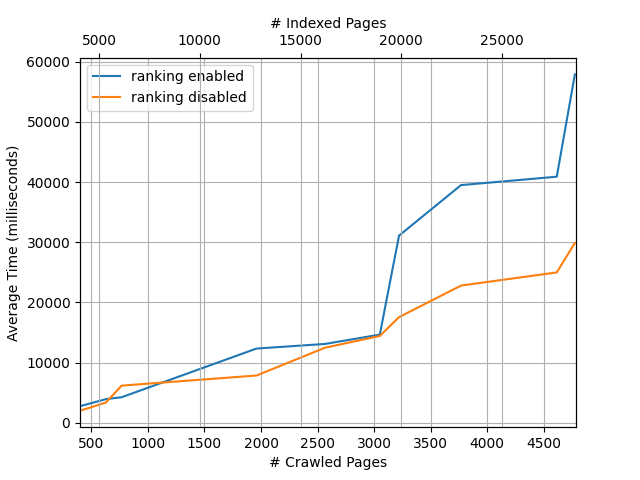
\includegraphics[width=15cm]{avgtime.png}
  \caption{Average Time vs. Num. Crawled Pages and Indexed keywords}
  \label{fig:avgtime}
\end{figure}

\begin{figure}
  \centering
  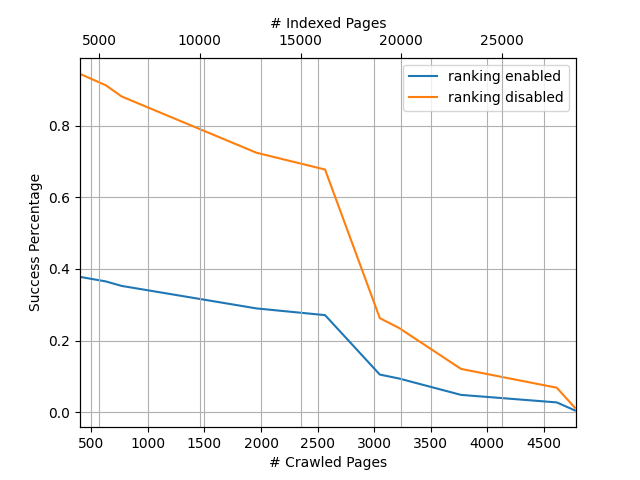
\includegraphics[width=15cm]{secPrec.png}
  \caption{Success Precentage vs. Num. Crawled Pages and Indexed keywords}
  \label{fig:secPrec}
\end{figure}

\clearpage

\section{Conclusion}
We notice that with the increase of indexed words and fetched documents, the performance slows down significantly, specially with ranking enabled.

\appendix
\section{JSON Outputs}
\begin{verbatim}
  {
    "avgTimeWithRanking": 2810,
    "successPercentageWithRanking": 0.3772932296296786,
    "totalParallelRequests": 200,
    "numCrawledPages": 410,
    "numIndexedKeywords": 4069,
    "avgTimeWithoutRanking": 2064,
    "successPercentageWithoutRanking": 0.9432330740741964
  }
  {
    "avgTimeWithRanking": 13477,
    "successPercentageWithRanking": 0.3669081310536714,
    "totalParallelRequests": 200,
    "numCrawledPages": 500,
    "numIndexedKeywords": 4945,
    "avgTimeWithoutRanking": 3618,
    "successPercentageWithoutRanking": 0.9172703276341785
  }
  {
    "avgTimeWithRanking": 4252,
    "successPercentageWithRanking": 0.3526412302053957,
    "totalParallelRequests": 200,
    "numCrawledPages": 768,
    "numIndexedKeywords": 7478,
    "avgTimeWithoutRanking": 6181,
    "successPercentageWithoutRanking": 0.8816030755134892
  }
  {
    "avgTimeWithRanking": 12340,
    "successPercentageWithRanking": 0.28977784909463156,
    "totalParallelRequests": 200,
    "numCrawledPages": 1960,
    "numIndexedKeywords": 8156,
    "avgTimeWithoutRanking": 7861,
    "successPercentageWithoutRanking": 0.7244446227365788
  }
  {
    "avgTimeWithRanking": 13108,
    "successPercentageWithRanking": 0.2710389771875954,
    "totalParallelRequests": 200,
    "numCrawledPages": 2566,
    "numIndexedKeywords": 14968,
    "avgTimeWithoutRanking": 12482,
    "successPercentageWithoutRanking": 0.6775974429689885
  }
  {
    "avgTimeWithRanking": 14653,
    "successPercentageWithRanking": 0.10506302696840852,
    "totalParallelRequests": 200,
    "numCrawledPages": 3050,
    "numIndexedKeywords": 19573,
    "avgTimeWithoutRanking": 14438,
    "successPercentageWithoutRanking": 0.2626575674210213
  }
  {
    "avgTimeWithRanking": 31112,
    "successPercentageWithRanking": 0.09406942826303775,
    "totalParallelRequests": 200,
    "numCrawledPages": 3220,
    "numIndexedKeywords": 19889,
    "avgTimeWithoutRanking": 17566,
    "successPercentageWithoutRanking": 0.23517357065759437
  }
  {
    "avgTimeWithRanking": 39504,
    "successPercentageWithRanking": 0.048332637200826284,
    "totalParallelRequests": 200,
    "numCrawledPages": 3768,
    "numIndexedKeywords": 24796,
    "avgTimeWithoutRanking": 22807,
    "successPercentageWithoutRanking": 0.1208315930020657
  }
  {
    "avgTimeWithRanking": 40900,
    "successPercentageWithRanking": 0.027352721400212988,
    "totalParallelRequests": 200,
    "numCrawledPages": 4614,
    "numIndexedKeywords": 25077,
    "avgTimeWithoutRanking": 24994,
    "successPercentageWithoutRanking": 0.06838180350053247
  }
  {
    "avgTimeWithRanking": 57899,
    "successPercentageWithRanking": 0.005037925670790111,
    "totalParallelRequests": 200,
    "numCrawledPages": 4774,
    "numIndexedKeywords": 28660,
    "avgTimeWithoutRanking": 29895,
    "successPercentageWithoutRanking": 0.012594814176975277
  }  
\end{verbatim}

\end{document}